\chapter{Preliminaries}
\label{chapter:prelims}




\section{Network dynamics}
\label{section:ch2_1}
\bigskip

The brain is a dynamical system, evolving continuously in response to external input and in
accordance with its own connectivity \cite{vogels2005neural,rajan2010stimulus,shenoy2011dynamical}.
Studying that relationship requires a model of it, and the model used here is the standard rate
description of a recurrent network \cite{breakspear2017dynamic,sussillo2014neural}. A neuron is
summarised by a single quantity, its membrane potential $x_i(t)$, which left alone decays
exponentially with time constant $\tau$. A neuron is rarely left alone. It receives a
time-dependent external input $I_i(t)$, and from each neuron $j$ that connects to it a current
$w_{ij}\phi(x_j)$, where $w_{ij}$ is the strength of the connection from $j$ to $i$, and $\phi$ converts
membrane potential into firing rate. Decay, recurrent input and external drive together give

\begin{equation}
    \tau \frac{\mathrm{d}x_i(t)}{\mathrm{d}t} = -x_i(t) + \sum_{j=1}^{N} w_{ij}\,\phi(x_j(t)) + I_i(t).
    \label{eq:membrane_potential}
\end{equation}

There is one such equation for every neuron, and each depends on the firing rates of all the others,
so none can be solved on its own. Stacking them into vectors gives a single equation for the
population as a whole,

\begin{equation}
    \tau \frac{\mathrm{d}\mathbf{x}(t)}{\mathrm{d}t} = -\mathbf{x}(t) + \mathbf{W}\boldsymbol{\phi}(\mathbf{x}(t)) + \mathbf{I}(t),
    \label{eq:vector_form}
\end{equation}

where $\mathbf{x}(t)$ holds the membrane potentials of all $N$ neurons, $\boldsymbol{\phi}$ is applied
element-wise, and $\mathbf{I}(t)$ is the external drive.

Written this way, the network's wiring occupies a single object. The connectivity matrix
$\mathbf{W} \in \mathbb{R}^{N \times N}$ collects every connection strength, with $w_{ij} = 0$
wherever no connection exists, and it is the only term in Equation~\ref{eq:vector_form} through
which structure can act. What it does there is multiply: at each instant $\mathbf{W}$ takes the
current pattern of firing rates and returns the recurrent contribution to every neuron's input,
acting as a linear map $\mathbf{W} : \mathbb{R}^{N} \to \mathbb{R}^{N}$. Whatever a wiring diagram
does to dynamics, it does through the repeated application of this map, and understanding the map is
therefore the whole of the problem.

Simulating the network requires discretising Equation~\ref{eq:vector_form}. Taking a forward Euler
step of size $\Delta t$, writing $\gamma = \Delta t / \tau$, and choosing $\phi = \tanh$ gives the
update used throughout this report,

\begin{equation}
    \mathbf{x}(t + 1) = (1 - \gamma)\,\mathbf{x}(t) + \gamma \tanh\!\left(\mathbf{W}\mathbf{x}(t) + \mathbf{W}_{\!\mathrm{in}}\mathbf{u}(t + 1)\right),
    \label{eq:reservoir_update}
\end{equation}

in which $\mathbf{u}(t)$ is the input signal at time $t$ and $\mathbf{W}_{\!\mathrm{in}}$ maps it
onto the network. Two conventions are worth noting. Following standard practice for rate networks,
the state is read directly as a firing rate and the nonlinearity is applied to the total input a unit
receives, rather than to each incoming current separately. And the leak rate $\gamma$ is the discrete
counterpart of the time constant, setting how much of the previous state carries over into the next
step: at $\gamma = 1$, the setting for every task here but one, the network advances by a full time
constant and Equation~\ref{eq:reservoir_update} reduces to
$\mathbf{x}(t+1) = \tanh(\mathbf{W}\mathbf{x}(t) + \mathbf{W}_{\!\mathrm{in}}\mathbf{u}(t+1))$.

We work in discrete time from here on, and the shift matters for what follows. In continuous time the
fate of a perturbation is governed by the real parts of the eigenvalues of $\mathbf{W}$; in discrete
time it is governed by their moduli.




\section{The spectrum of a connectivity matrix}
\label{section:ch2_2}
\bigskip

To see what the wiring alone contributes, it helps to strip away everything else. With the input set
to zero and $\phi$ taken to be the identity, Equation~\ref{eq:reservoir_update} collapses to the linear
map $\mathbf{x}(t+1) = \mathbf{W}\mathbf{x}(t)$, so that the state after $t$ steps is simply
$\mathbf{W}^{t}\mathbf{x}(0)$. The behaviour of the network becomes a question about a single
matrix: what does applying $\mathbf{W}$ over and over do to a vector? The eigendecomposition answers
it. Provided its eigenvectors are linearly independent, which holds for almost every matrix,
$\mathbf{W} = \mathbf{V}\boldsymbol{\Lambda}\mathbf{V}^{-1}$, where the columns of $\mathbf{V}$ are the
eigenvectors $\mathbf{v}_i$ satisfying $\mathbf{W}\mathbf{v}_i = \lambda_i\mathbf{v}_i$, and
$\boldsymbol{\Lambda}$ is diagonal with the eigenvalues $\lambda_i$ along it. The set of eigenvalues is the
\textbf{eigenspectrum}, or simply the \say{spectrum}.

This decomposition is useful here because of what an eigenvector means for a population of neurons.
A vector in $\mathbb{R}^{N}$ is a pattern of activity across that population, and an eigenvector is a
pattern the connectivity gives back unchanged apart from its amplitude. The neurons involved keep
their relative activation and so are locked together, rising and falling as a unit. Such patterns are
called \textbf{modes}, and a neuron may belong to many of them at once. Expressed in the basis of
modes, $\mathbf{c}(t) = \mathbf{V}^{-1}\mathbf{x}(t)$, the network's dynamics come apart into $N$
independent scalar equations, $c_i(t+1) = \lambda_i c_i(t)$, each solved by
$c_i(t) = \lambda_i^{t}\,c_i(0)$. The activity of the network is their superposition,

\begin{equation}
    \mathbf{x}(t) = \sum_{i=1}^{N} \lambda_i^{t}\;c_i(0)\,\mathbf{v}_i.
    \label{eq:mode_superposition}
\end{equation}

A coupled network of $N$ neurons has become $N$ uncoupled patterns, each evolving on its own, and the
entire fate of a pattern is settled by one number. 
Complex eigenvalues arrive in conjugate pairs whose combination is a rotation, producing
oscillation rather than monotonic growth or decay.
That reduction is what makes the spectrum worth studying in its own right. 
It is computed from the wiring alone, before anything is simulated, yet it already fixes how activity 
behaves (Figure~\ref{fig:Eigenspectra-dynamics}). So, what can we learn about the dynamics of the network 
from simply analysing the connectivity matrix's eigenspectrum?

\begin{keyideas}[What the spectrum tells us about the dynamics]
    \item \textbf{Stability and dynamical regime.} A mode evolves as $\lambda_i^{t}$, so it decays
    if $|\lambda_i| < 1$ and grows if $|\lambda_i| > 1$. The network is stable when this holds for
    every mode, and above that threshold at least one pattern sustains or amplifies itself, so that
    activity is increasingly dictated by the network's own feedback rather than by what it is given.

    \item \textbf{Timescales.} The modulus of an eigenvalue sets how quickly its mode decays, so the
    spectrum is a catalogue of the timescales a network can support. Where eigenvalues cluster, many
    modes share a timescale and are liable to respond in synchrony \cite{rajan2006eigenvalue}.

    \item \textbf{Dominant directions.} An eigenvalue whose modulus clearly exceeds the rest belongs
    to a mode that outlives every other, and so governs the network's long-run behaviour. What sets
    its influence is not its size but its separation from the rest of the spectrum.
\end{keyideas}

% Eigenspectrum dynamics schematic
\begin{figure}[ht]
    \centering
    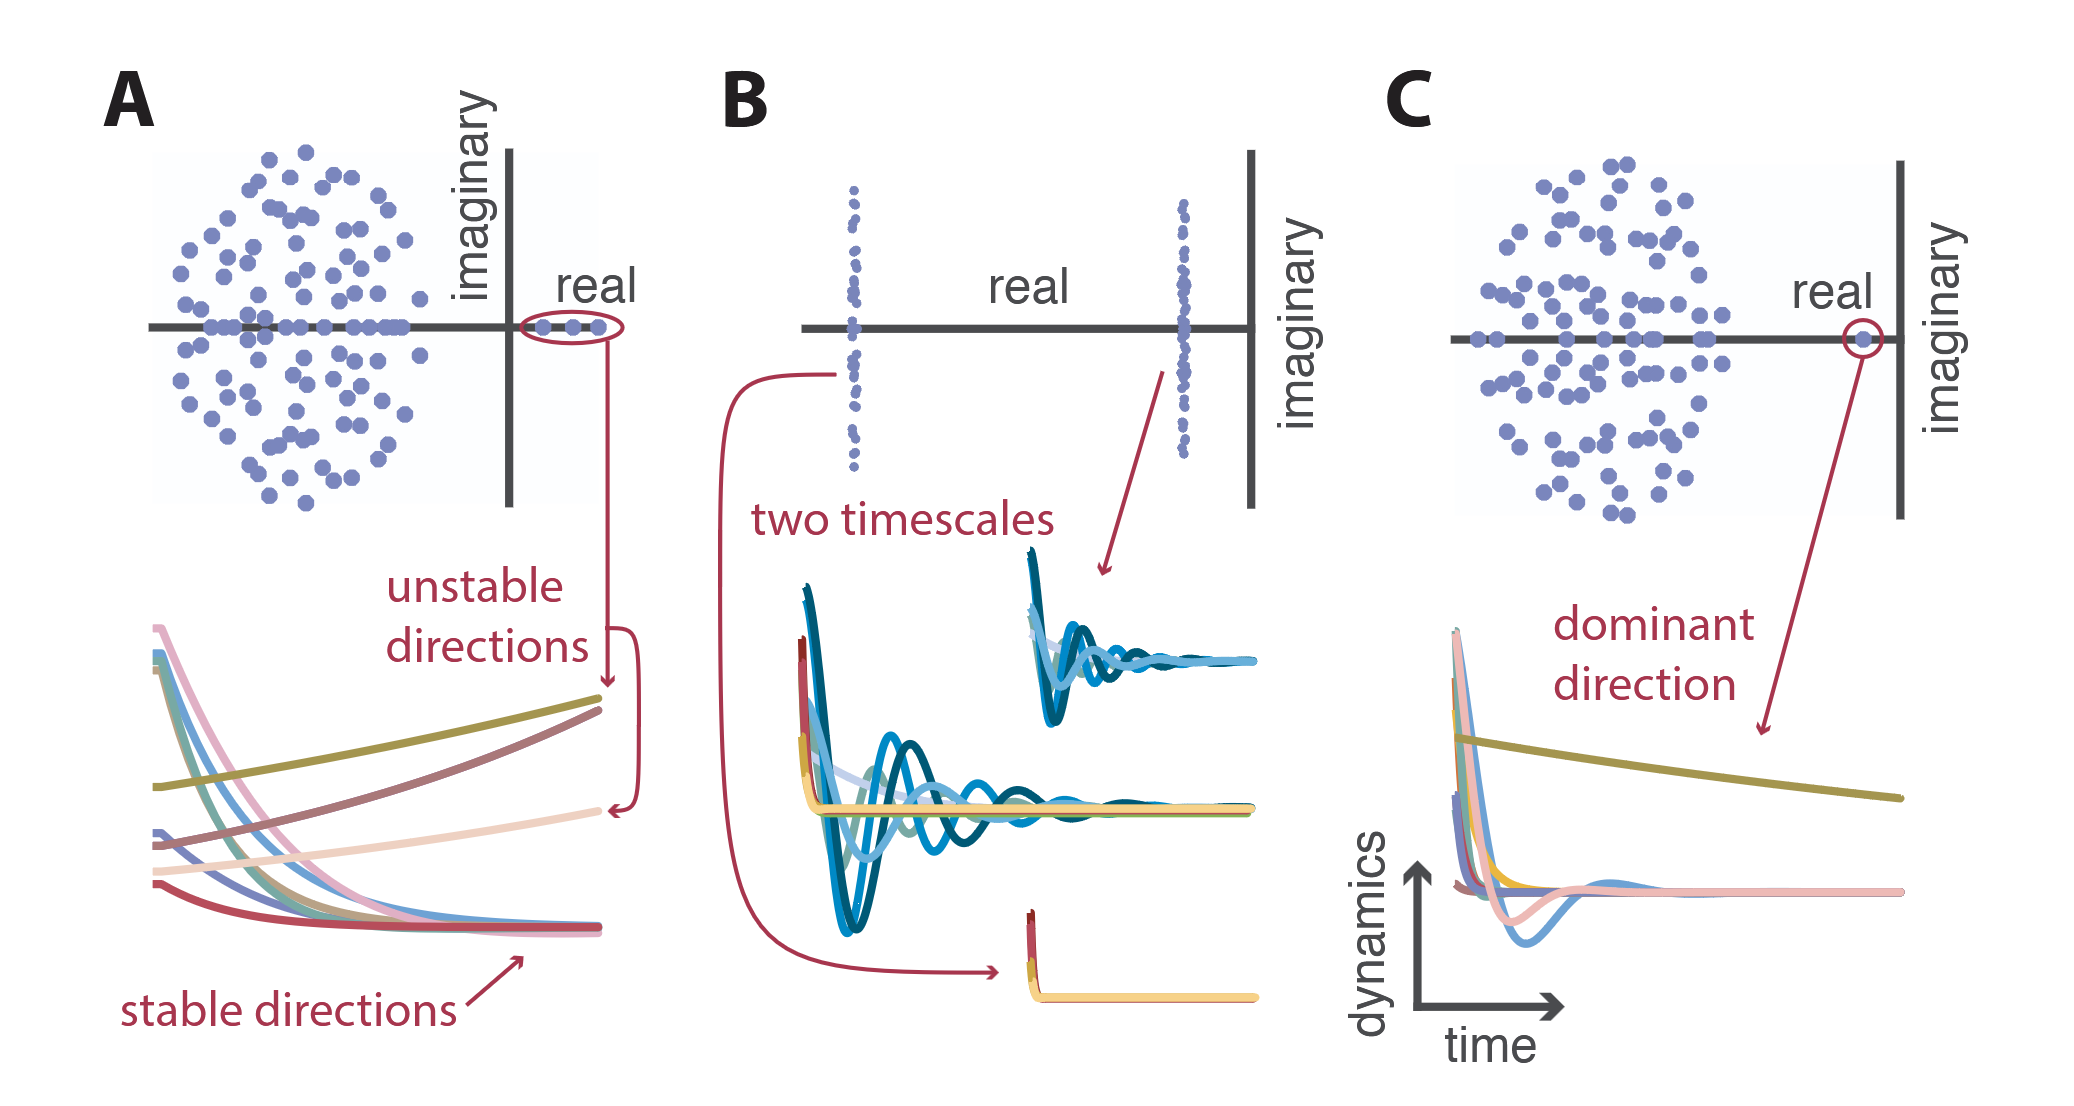
\includegraphics[width=0.8\textwidth]{figures/Eigenspectrum-dynamics.png}
    \caption[What the spectrum tells us about dynamics]{%
    \textbf{What the spectrum tells us about dynamics.}
    \textbf{(a)} Stability. Spectra at three operating points, with the unit circle marked, and the
    activity each produces: below $\rho(\mathbf{W}) = 1$ a perturbation decays, at one it is sustained,
    above one it grows.
    \textbf{(b)} Timescales. Two spectra of equal radius but different arrangement. Clustered
    eigenvalues give modes that decay together, producing synchronised activity; spread eigenvalues
    give staggered decay across a range of timescales.
    \textbf{(c)} Dominant directions. Two spectra sharing a leading eigenvalue but differing in their
    separation from the bulk, with the resulting activity decomposed into the leading mode and the
    remainder. A large gap leaves the leading mode governing the response almost alone; a small one
    leaves activity distributed across many modes.}
    \label{fig:Eigenspectra-dynamics}
\end{figure}

The first point above gives us a control. The threshold is the \textbf{spectral radius}
$\rho(\mathbf{W}) = \operatorname{max}_i|\lambda_i|$, the modulus of the largest eigenvalue: below one,
perturbations die away and the network eventually forgets its initial condition; above one, they do
not. Because every eigenvalue scales with the weights, multiplying $\mathbf{W}$ by a constant slides
the whole spectrum in or out without disturbing its internal arrangement. Rescaling in this way is
how a network's dynamical state is set, and the value it is rescaled to, written $\sigma$, is what we
call its \textbf{operating point}. It is also what makes structures comparable: two networks placed
at the same operating point differ in the shape of their spectra rather than in its overall size.

The third gives us the object of study. Separating the largest eigenvalue $\lambda_1$ from the
\textbf{bulk} of eigenvalues beneath it splits the spectrum into two parts with different roles. The
first is the part we rescale, and therefore control. The second is where a network's particular
wiring leaves its mark. What matters is how far apart they sit, since after $t$ steps the leading
mode is amplified relative to another by $(|\lambda_1|/|\lambda_i|)^{t}$: a network whose leading
eigenvalue stands well clear of its bulk spends its activity on one shared pattern, while a network
whose spectrum is more even spreads it across many. We refer to this separation as the
\textbf{spectral gap}, and quantify it as a ratio in Chapter~\ref{chapter:methods}
\cite{schaub2015emergence}.

The connectomes studied here make that division especially clean. Reconstructed from streamline
counts, their weights are non-negative, and the Perron--Frobenius theorem then guarantees that the
largest eigenvalue is real, positive and equal to the spectral radius, with an eigenvector that can
be chosen non-negative throughout. The dominant mode of a non-negative network is therefore a pattern
in which every neuron participates with the same sign: a \textbf{common mode} shared by the whole
population rather than a contrast between one part of it and another. Separately, the macroscale
connectome is symmetric by construction, which makes $\mathbf{W}$ normal, its spectrum real and its
eigenvectors mutually orthogonal.

That last property is convenient but not generic, and where it fails the spectrum stops being the
whole story. Diagonalising a matrix implicitly treats its eigenvectors as an orthonormal basis and in
doing so discards how they are oriented relative to one another, so two matrices with identical
spectra may still behave differently. When eigenvectors overlap, activity along one mode leaks into
another, and a network can amplify a perturbation transiently even though every eigenvalue predicts
decay. The spectrum bounds the asymptotic behaviour but not the transient. Any manipulation that
breaks the symmetry of $\mathbf{W}$ therefore introduces this effect alongside whatever else it was
intended to do, a point we return to when weights are given signs.









\section{Reservoir computing}
\label{section:ch2_3}
\bigskip

Reservoir computing puts a network of this kind to work on a task
\cite{jaeger2001echo,maass2002real,lukovsevivcius2009reservoir}. The architecture has three parts
(Figure~\ref{fig:RC}c). An input layer projects a signal $\mathbf{u}(t)$ onto the network through a
fixed matrix $\mathbf{W}_{\!\mathrm{in}}$, whose entries are drawn at random from $\{-1, +1\}$ and
scaled by a task-specific constant; unless stated otherwise every unit receives input, so that no
part of the network is privileged by the way the signal enters it. A recurrent layer, the
\textbf{reservoir}, evolves according to Equation~\ref{eq:reservoir_update}, carrying the input
forward as a high-dimensional trajectory that retains a nonlinear record of what the network has
recently been given. An output layer reads that trajectory out. Only the last of the three is
trained: $\mathbf{W}_{\!\mathrm{in}}$ and $\mathbf{W}$ are generated once and thereafter left alone.

% Reservoir Computing schematic
\begin{figure}[ht]
    \centering
    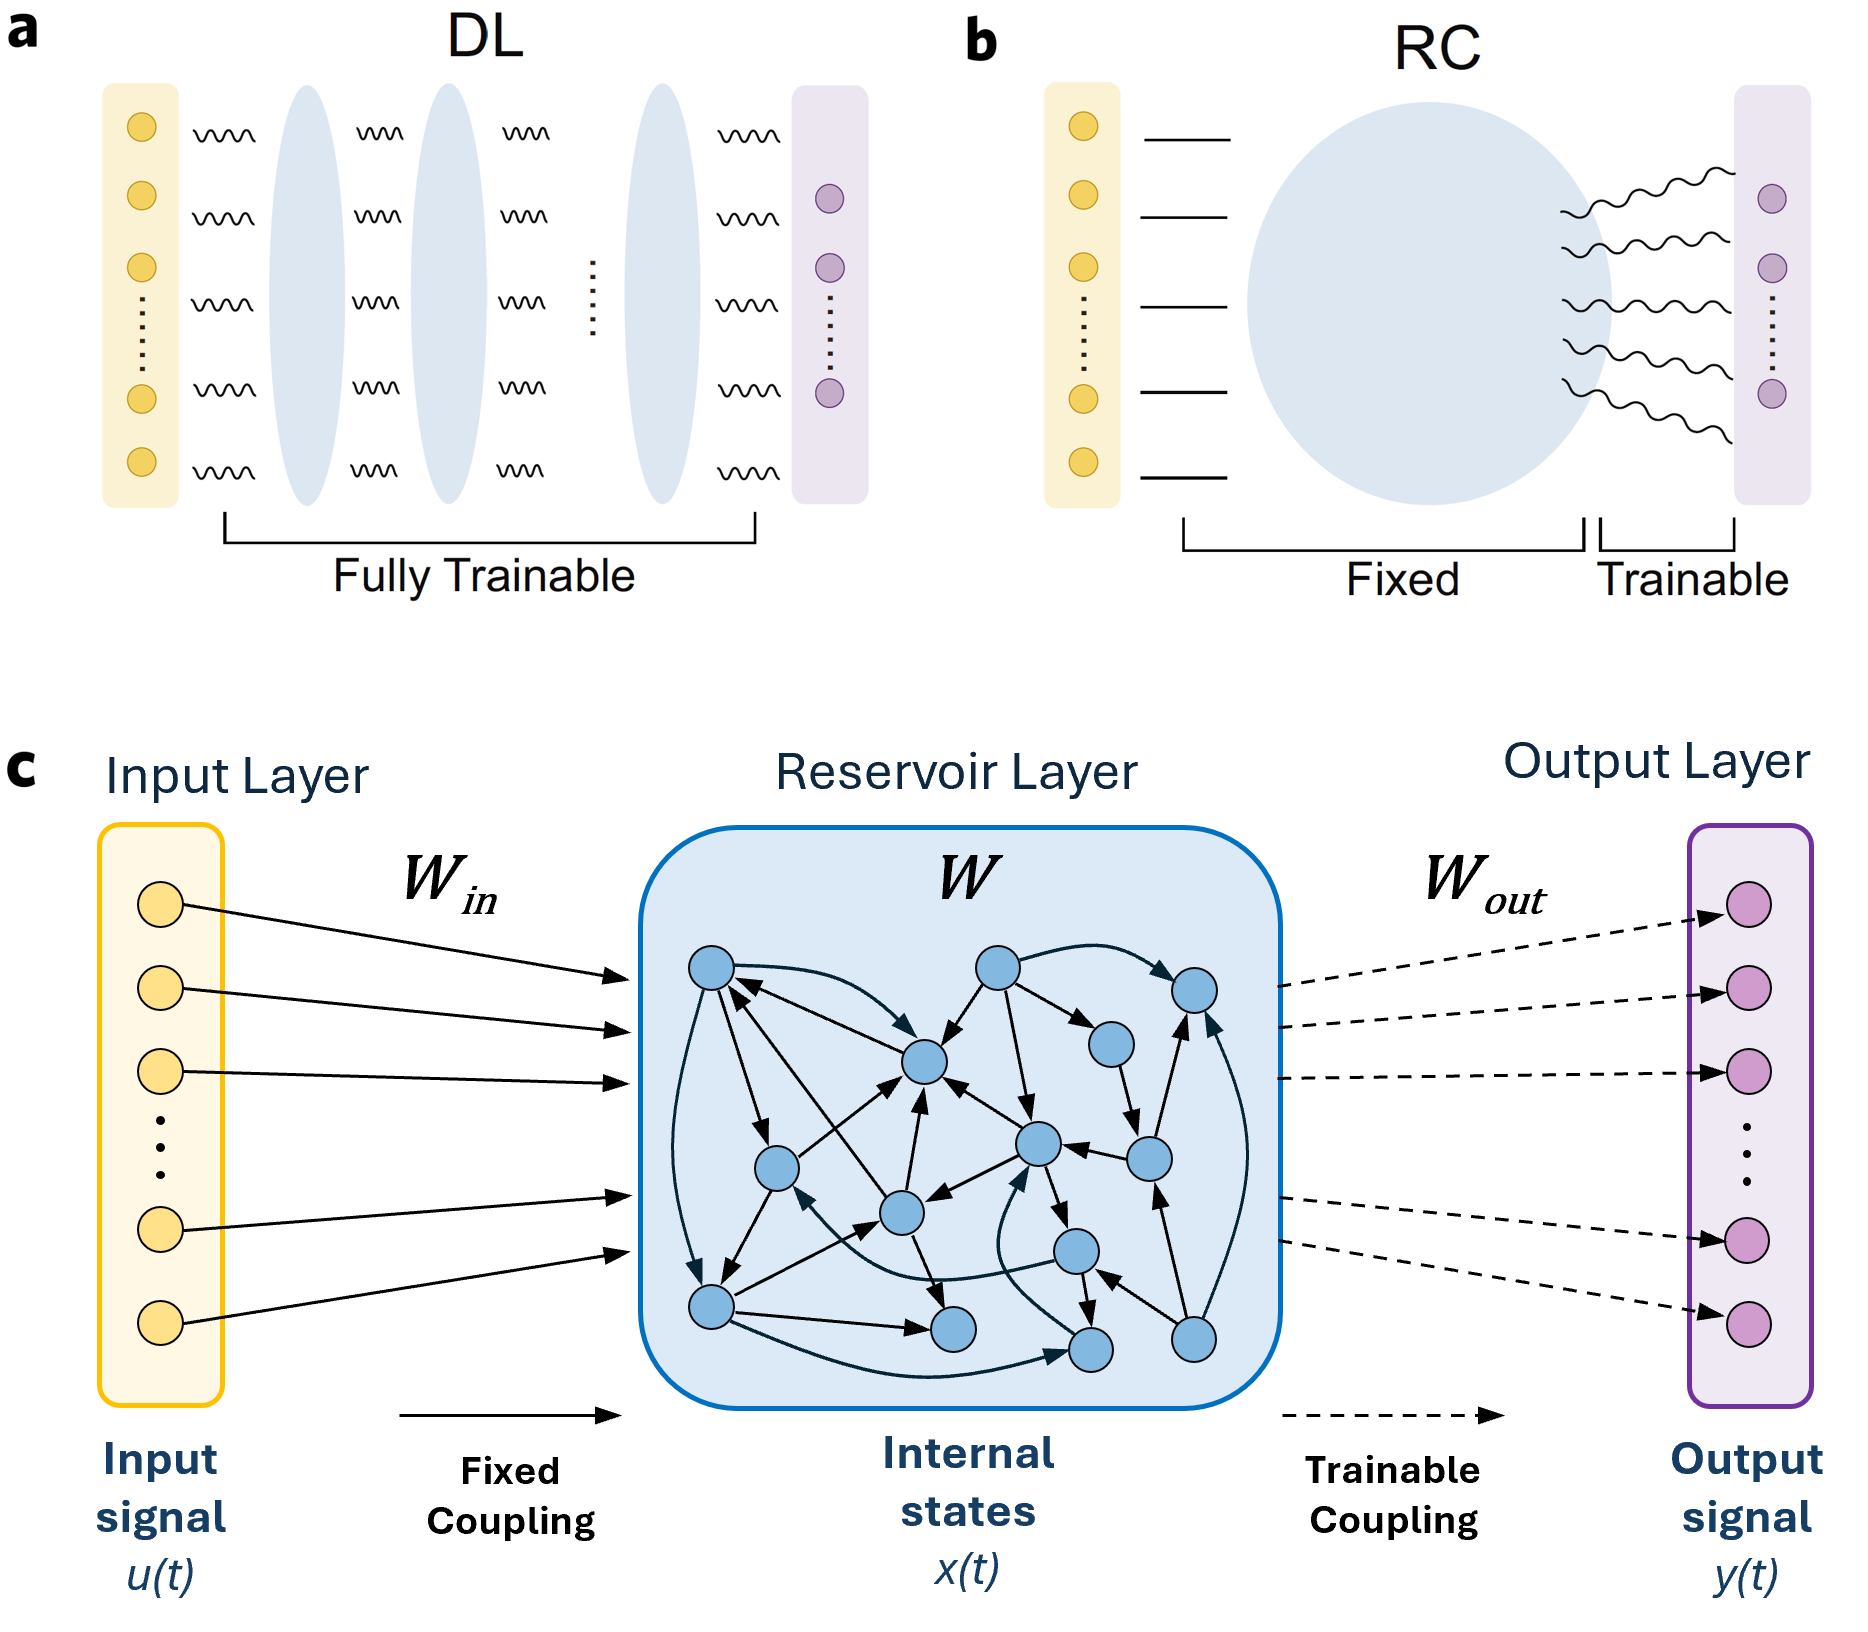
\includegraphics[width=0.9\textwidth]{figures/ReservoirComputing.png}
    \caption[Reservoir computing]{%
    \textbf{Reservoir computing.} A reservoir differs from a conventional deep network in what is
    trained rather than in what it computes.
    \textbf{(a)} In a deep network every connection is learned, shown here as wavy lines.
    \textbf{(b)} In a reservoir only the readout weights are learned; the input and recurrent
    connections are generated once and then held fixed, shown as straight lines.
    \textbf{(c)} Input and output are time series, $\mathbf{u}(t)$ and $\mathbf{y}(t)$. The input is
    projected onto a recurrent network whose state evolves according to
    Equation~\ref{eq:reservoir_update}, and the readout recombines that state linearly to produce the
    output. Because the recurrent weights are fixed, the connectivity under test survives training
    unchanged. Figure adapted from \cite{yan2024emerging}.}
    \label{fig:RC}
\end{figure}

The readout is a linear map from the state to the target signal, so that the prediction at time $t$
is $\mathbf{x}(t)^{\top}\mathbf{W}_{\!\mathrm{out}}$. Collecting the $T$ states visited during a run
into the rows of a state matrix $\mathbf{A} \in \mathbb{R}^{T \times N}$, and the corresponding targets into
$\mathbf{Y} \in \mathbb{R}^{T \times n_y}$, the readout weights are those minimising squared error with a
penalty on their size,

\begin{equation}
    \mathbf{W}_{\!\mathrm{out}} = \arg\min_{\mathbf{W}} \; \lVert \mathbf{A}\mathbf{W} - \mathbf{Y} \rVert_{F}^{2} + \alpha \lVert \mathbf{W} \rVert_{F}^{2}
    \; = \; (\mathbf{A}^{\top}\mathbf{A} + \alpha \mathbf{I}_N)^{-1}\mathbf{A}^{\top}\mathbf{Y}.
    \label{eq:ridge}
\end{equation}

This is ridge regression. The closed form on the right makes training a single linear solve rather
than an iterative optimisation, which is what makes it practical to fit many thousands of networks
across a range of structures and operating points. The regularisation
strength $\alpha$ decides how faint a direction of activity the readout is willing to lean on: a
direction is useful to it only insofar as the network's activity along that direction stands above
$\alpha$. It enters here as a numerical safeguard against inverting a near-singular matrix, but it
turns out to do more than that, and we return to it in Chapter~\ref{chapter:methods}. The matrix
being inverted, $\mathbf{A}^{\top}\mathbf{A}$, is the \textbf{Gram matrix} of the states, and we will have cause to
look at its spectrum directly.

This arrangement is what makes the hypothesis of Chapter~\ref{chapter:introduction} testable. Because
the recurrent weights are never updated, any connectivity pattern we choose can be imposed on the
network and is guaranteed to survive training intact. A difference in performance between two
reservoirs is then attributable to the wiring they were given, and not to what training made of it.
The dynamical state is equally under our control: rescaling $\mathbf{W}$ moves a network through the
regimes of Section~\ref{section:ch2_2}, so structures can be compared at matched operating points,
and performance measured as a curve across them rather than as a single number. Structure and
dynamical state can therefore be varied independently, which is exactly what is needed to ask what
each contributes.

None of this makes a reservoir a model of how the brain learns. The readout is an instrument for
asking what a network's activity contains, not a claim about how the brain reads its own activity
out, and we take up the question of what these networks do and do not model in
Chapter~\ref{chapter:discussion}. What the framework offers is a controlled comparison: two networks
given the same input at the same operating point, differing only in how they are wired, and a
readout applied identically to both. Whatever separates their performance is attributable to connectivity, 
and we can ask what that wiring is worth.




\section{The geometry of activity}
\label{section:ch2_4}
\bigskip

The spectrum tells us what a network does with a perturbation. A network performing a task, however,
is not perturbed once and then left to settle: it is driven continuously, and what the readout sees
is the trajectory that driving produces. Over a run of $T$ steps the state visits $T$ points in
$\mathbb{R}^{N}$, and those points are not scattered arbitrarily. Every one is produced from the last
by the same map, so the trajectory is confined to a structured region of the state space whose shape
is a joint property of the connectivity and the input. It is this shape, and not $\mathbf{W}$ itself,
that the readout has access to. Describing it geometrically is a well-established way of relating
population activity to computation \cite{chung2021neural,vyas2020computation}.

The most basic question to ask of a shape is how many dimensions it occupies. If activity is confined
to a handful of directions then, however many units the network has, the readout is choosing among
correspondingly few signals; if it extends into many, there is more for the readout to combine.
Dimensionality in this sense is not the rank of the state matrix $\mathbf{A}$, which for a nonlinear network
is almost always full. It is a graded measure of how the trajectory's variation is distributed across
directions, computed from the eigenvalues of the Gram matrix $\mathbf{G}$ met in the previous section, or of
the state covariance.

Any such measure has to decide how much a direction counts for, and that decision is not innocuous.
The obvious choice is to weight by variance, counting a direction in proportion to how much of the
activity's movement it accounts for. But Equation~\ref{eq:ridge} shows this is not the weighting the
readout applies. Ridge regression discounts a direction according to how its Gram eigenvalue compares
with $\alpha$, so a direction carrying very little of the activity remains available provided it is
not so small as to be suppressed by the regularisation. A measure weighted by variance and a measure
weighted by what a readout can recover therefore need not agree. The two also rest on different
matrices, since a variance-based measure is computed after each unit's mean over time has been
removed, whereas a readout is fitted on the states themselves; on a network whose dominant pattern is
carried in those means, the two need not even be counting the same directions. The specific measures
used in this report are defined in Chapter~\ref{chapter:methods}. What matters here is that a
network's activity has a shape, that the shape has a size, and that its size depends on what is
reading it.

This completes the chain the report follows. Structure enters the dynamics through $\mathbf{W}$ and
nowhere else. The spectrum of $\mathbf{W}$ is computable from the wiring alone, before anything is
simulated, and yet already describes how activity will behave: which patterns persist, on what
timescales, and how much of the network's activity is claimed by a single dominant mode. It is in
this sense the natural midpoint between a static connectivity matrix and the dynamics that matrix
generates, belonging fully to neither. Driving such a network produces a trajectory whose geometry
inherits that spectral structure, and it is the geometry, not the wiring diagram, that determines
what a linear readout can extract from it. Structure sets the spectrum, the spectrum shapes the
geometry of activity, and that geometry governs what the network can compute. The chapters that
follow take these links one at a time.




\afterpage{\blankpage}